\chapter{Maximum Likelihood Estimation for Multiparameter Models}\label{S:MultiParamEst}

\section{Introduction}\label{S:MultiParamEstIntro}
When two or more parameters index a statistical experiment we want to estimate the vector-valued parameter $\theta^* := (\theta^*_1,\ldots,\theta^*_k)$.
Here we will find the maximum likelihood estimates of vector-valued parameters.  

The maximum likelihood estimator (MLE) of a possibly unknown but fixed parameter  $\theta^* := (\theta^*_1,\ldots,\theta^*_k)$  in a multi-parametric experiment, i.e.~$\theta^* \in \BB{\Theta} \subset \Rz^k$ with $1 < k < \infty$ is defined analogously to \hyperref[D:LklFn]{Definition~\ref*{D:MLE}} with the exception that we allow the parameter to be a vector.  We take an excursion in multi-dimensional optimisation before finding the MLE of a parametric experiment involving two parameters.

 \section{Practical Excursion in Multi-dimensional Optimisation}\label{S:PracticalMultiDimOptimization}
The basic idea involves multi-dimensional iterations that attempt to converge on a local maximum close to the starting vector $\theta^{(0)} \in \BB{\Theta}$ (our initial guess).  We can employ {\sc Matlab}'s built-in function {\tt fminsearch} to find the MLE of vector-valued parameters such as in the $\lognormal$ model with two parameters, i.e.~$\theta=(\lambda,\zeta) \in \BB{\Theta} \subset \Rz^2$.  The  function {\tt fminsearch} is similar to {\tt fminbnd} except that it handles a given function of many variables, and the user specifies a starting vector $\theta^{(0)}$ rather than a starting interval.  Thus, {\tt fminsearch} tries to return a vector $\theta^{(*)}$ that is a local minimiser of, $-\log(L(x_1,x_2,\ldots,x_n; \theta)$, the negative log-likelihood function of the vector-valued parameter $\theta$, near this starting vector $\theta^{(0)}$.  
We illustrate the use of {\tt fminsearch} on a more challenging target called the Levy density:

{\scriptsize
\begin{equation}\label{E:LevyDensity}
f(x,y)   =  \exp \left(-\frac{1}{50} \left( \left( \sum_{i=1}^5 {i \cos{((i-1)x+i)} } \right) \left( \sum_{j=1}^5 {j \cos{((j+1)y+j)} } \right)+ (x + 1.42513 )^2 + (y + 0.80032)^2\right) \right)
\end{equation}
}

\begin{figure}[htpb]
\caption{Plot of Levy density as a function of the parameter $(x,y) \in [-10,10]^2$ scripted in \hyperref[Mf:LevyDensityPlot]{Labwork \ref*{Mf:LevyDensityPlot}}.\label {F:LevyDensityPlot}}
\begin{center}
\makebox{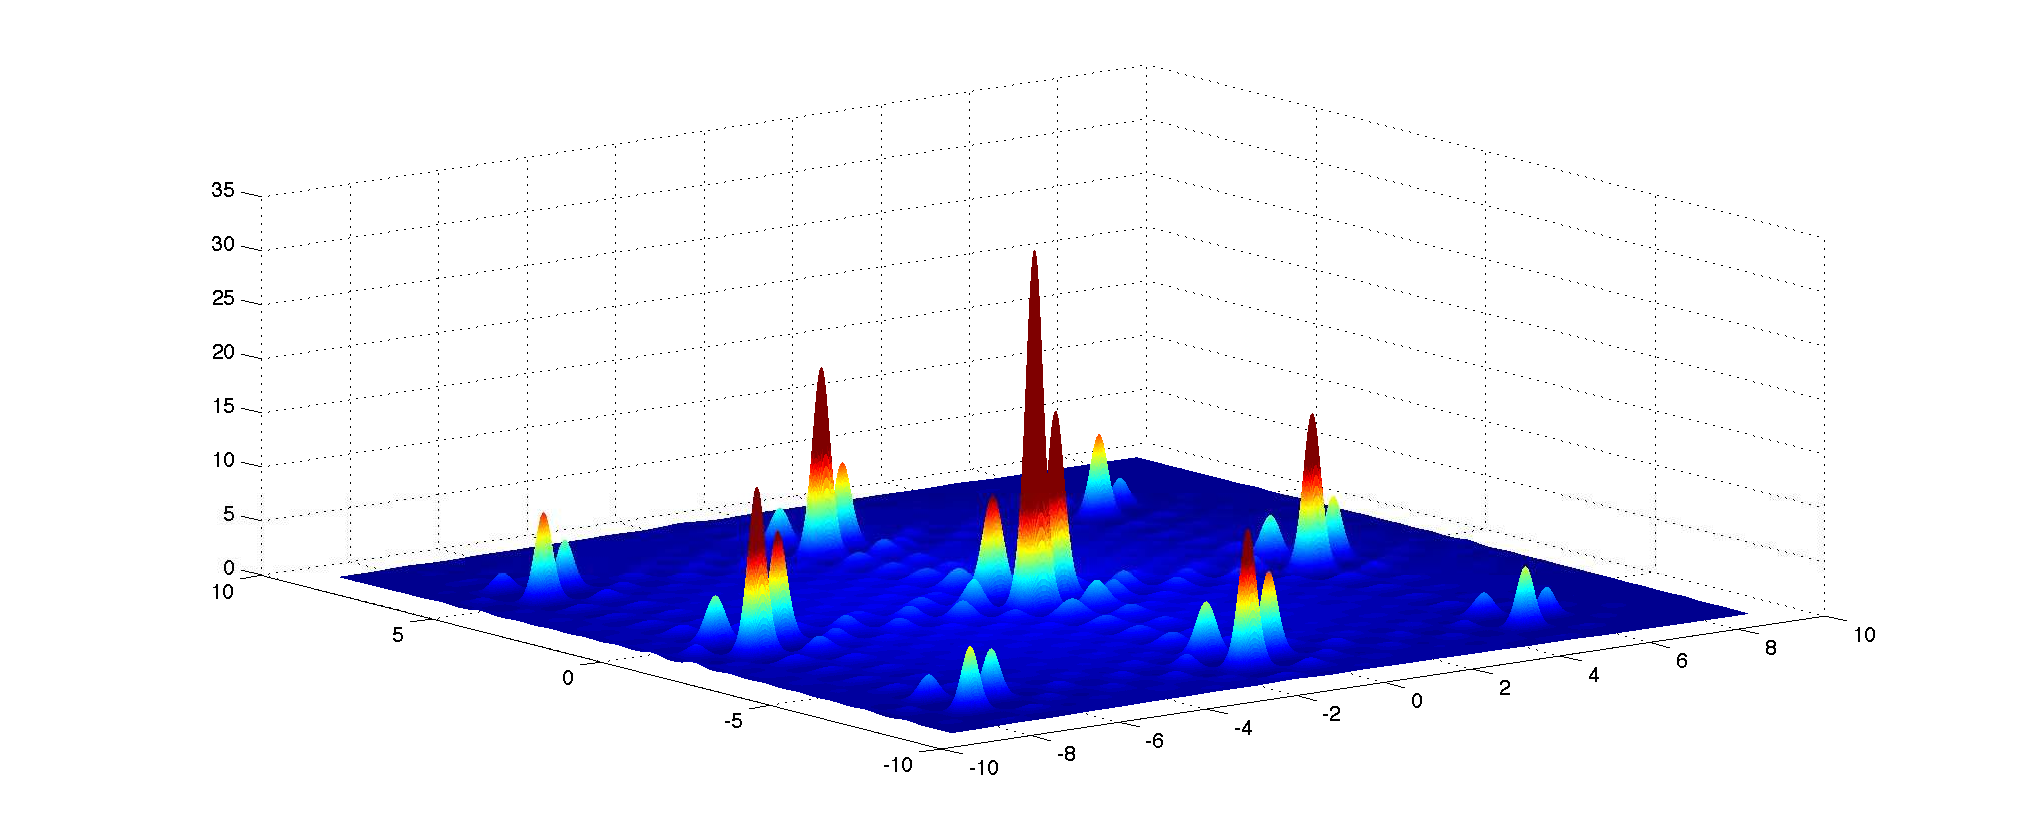
\includegraphics[width=6.750in]{figures/LevyDensityT50}}
\end{center}
\end{figure}

{\tt fminsearch} uses the simplex search method [Nelder, J.A., and Mead, R.~1965, Computer Journal, vol.~7, p.~308-313].  For an animation of the method and more details, please visit \href{http://en.wikipedia.org/wiki/Nelder-Mead_method}{\url{http://en.wikipedia.org/wiki/Nelder-Mead_method}}.  
%For a more recent treatment see Lagarias, J.C., J. A. Reeds, M. H. Wright, and P. E. Wright, {\em Convergence Properties of the Nelder-Mead Simplex Method in Low Dimensions}, SIAM Journal of Optimisation, Vol. 9 Number 1, pp. 112-147, 1998.  
An advantage of the method is that it does not use numerical (finite differencing) or analytical (closed-form expressions) gradients but relies on a direct search method.  Briefly, the simplex algorithm tries to ``tumble and shrink'' a simplex towards the local valley of the function to be minimised.  If $k$ is the dimension of the parameter space or domain of the function to be optimised, a $k$-dimensional simplex is specified by its $k+1$ distinct vertices each of dimension $k$.  Thus, a simplex is a triangle in a two-dimensional space and a pyramid in a three-dimensional space. At each iteration of the algorithm: 
\begin{enumerate}
\item A new point inside or nearby the current simplex is proposed.
\item The function's value at the newly proposed point is compared with its values at the vertices of the simplex. 
\item One of the vertices is typically replaced by the proposed point, giving rise to a new simplex. 
\item The first three steps are repeated until the diameter of the simplex is less than the specified tolerance.  
\end{enumerate}

A major limitation of {\tt fminsearch}, as demonstrated with the Levy target (encoded in \hyperref[Mf:NegLevyDensity]{Labwork~\ref*{Mf:NegLevyDensity}}) is that it  can only give local solutions.  The {\bf global maximiser} of the Levy function $f(x,y)$ is $(-1.3069, -1.4249)$ and the {\bf global maximum} is $f (-1.3069, -1.4249)=33.8775$ For instance, if we start the search close to, say $(x^{(0)},y^{(0)})=(-1.3,-1.4)$, as shown below, then the simplex algorithm converges as desired to the solution $(-1.3068, -1.4249)$.
\begin{VrbM}
>> [params, fvalue, exitflag, output] = fminsearch('NegLevyDensity',[-1.3 -1.4],options)
params =   -1.3068   -1.4249
fvalue =  -33.8775
exitflag =     1
output = 
    iterations: 24
     funcCount: 46
     algorithm: 'Nelder-Mead simplex direct search'
       message: [1x194 char]
\end{VrbM}
However, if we start the search further away, say $(x^{(0)},y^{(0)})=(1.3,1.4)$, as shown below, then the algorithm converges to the {\bf local maximiser} $(1.1627,1.3093)$ with a {\bf local maximum} value of $f(1.1627,1.3093)=0.9632$, which is clearly smaller than the global maximum of $33.8775$.  
\begin{VrbM}
>> [params, fvalue, exitflag, output] = fminsearch('NegLevyDensity',[1.3 1.4],options)
params = 1.1627    1.3093
fvalue = -0.9632
exitflag = 1
output = 
   iterations: 29
     funcCount: 57
     algorithm: 'Nelder-Mead simplex direct search'
       message: [1x194 char]
\end{VrbM}
Therefore, we have to be extremely careful when using point-valued, iterative,  local optimisation algorithms, implemented in floating-point arithmetic to find the global maximum.  Other examples of such algorithms include:
\begin{itemize}
\item {\bf Conjugate Gradient Method}:\\ \href{http://en.wikipedia.org/wiki/Conjugate_gradient_method}{\url{http://en.wikipedia.org/wiki/Conjugate_gradient_method}}
\item {\bf Broyden-Fletcher-Goldfarb-Shanno (BFGS) method}:\\ \href{http://en.wikipedia.org/wiki/BFGS_method}{\url{http://en.wikipedia.org/wiki/BFGS_method}}
\item {\bf Simulated Annealing}:\\ \href{http://en.wikipedia.org/wiki/Simulated_annealing}{\url{http://en.wikipedia.org/wiki/Simulated_annealing}}
\end{itemize}
In general, we have no guarantee that the output of such local optimisation routines will indeed be the global optimum.  In practice, you can start the search at several distinct starting points and choose the best local maximum from the lot.

\begin{figure}[hbpt]
\caption{Plot of the ``well-behaved'' (uni-modal and non-spiky) $\log(L((x_1,x_2,\ldots,x_{100});\lambda,\zeta))$, based on $100$ samples $(x_1,x_2,\ldots,x_{100})$ drawn from the $\lognormal(\lambda^*=10.36,\zeta^*=0.26)$ as per \hyperref[Mf:LogNormalLogLklPlot]{Labwork \ref*{Mf:LogNormalLogLklPlot}}.\label {F:LogNormalLogLklPlot}}
\begin{center}
\makebox{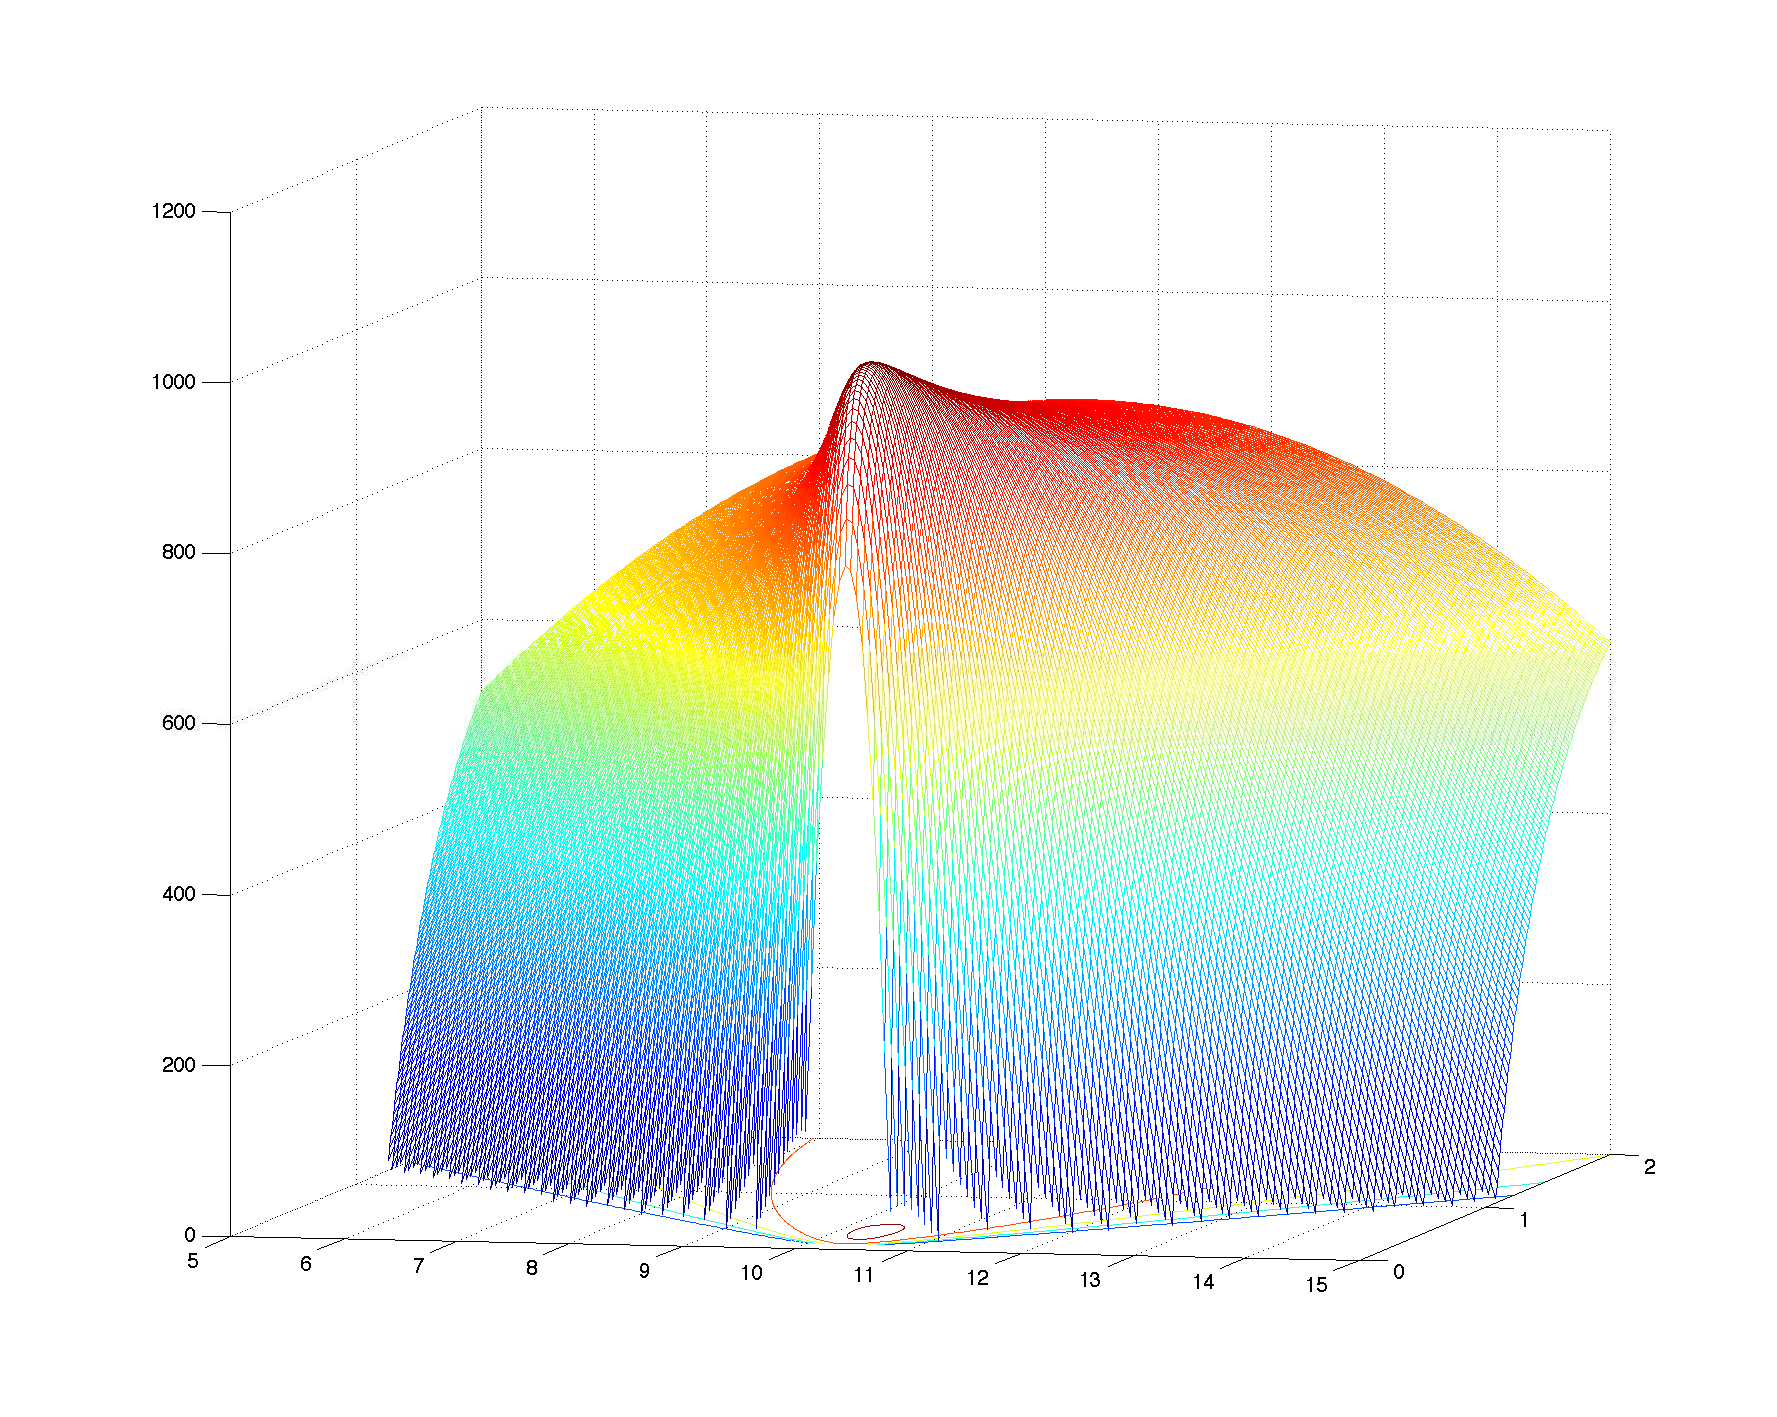
\includegraphics[width=4.0in]{figures/LogNormalLogLklPlot}}
\end{center}
\end{figure}

When the target function is ``well-behaved,'' i.e.~uni-modal or single-peaked and not too spiky, the optimisation routine can be expected to perform well.  Log-likelihood functions are often well-behaved.  Let us generate $100$ samples from an RV $C\sim \lognormal(\lambda^*=10.36, \zeta^*=0.26)$ by exponentiating the samples from the $\normal(10.36,0.26^2)$ RV, and then compute the corresponding MMEs and MLEs for parameters $(\lambda,\zeta)$ using the formulae in \hyperref[T:MMEMLE]{Table~\ref*{T:MMEMLE}}.
\begin{VrbM}
>> rand('twister',001); % set the fundamental sampler
>> % draw 100 samples from the Lognormal(10.36,0.26) RV
>> Cs = exp(arrayfun(@(u)(Sample1NormalByNewRap(u,10.36,0.26^2)),rand(1,100))); 
>> MLElambdahat = mean(log(Cs)) % maximum likelihood estimate of lambda 
MLElambdahat =   10.3397
>> MLEzetahat = sqrt(mean( (log(Cs)-MLElambdahat) .^ 2)) % max. lkl. estimate of zeta
MLEzetahat =    0.2744
>> MMEzetaahat = sqrt(log(var(Cs)/(mean(Cs)^2) + 1)) % moment estimate of zeta
MMEzetaahat =    0.2624
>> MMElambdahat = log(mean(Cs))-(0.5*MMEzetaahat^2) % moment estimate of lambda
MMElambdahat =   10.3417
\end{VrbM}
Let us try to apply the simplex algorithm to find the MLE numerically.  We first encode the negative log-likelihood function of the parameters $(\lambda,\zeta) \in (0,\infty)^2$ for the given data $x$, as follows: 
{\VrbMf[label=NegLogNormalLogLkl.m]{scripts/NegLogNormalLogLkl.m}}
Here is how we can call {\tt fminsearch} and find the MLE after the re-transformation. 
\begin{VrbM}
>> [params, fvalue, exitflag, output] = ...
fminsearch(@(params)(NegLogNormalLogLkl(Cs,params)),[log(5), log(1)])
params =    2.3360   -1.2931
fvalue =  -1.0214e+03
exitflag =     1
output = 
    iterations: 74
     funcCount: 131
     algorithm: 'Nelder-Mead simplex direct search'
       message: [1x194 char]
>> % But we want exp(params) since we defined lambda and zeta as exp(params)
exp(params)
ans =   10.3397    0.2744
\end{VrbM}
Note that the MLEs $(\widehat{\lambda}_{100},\widehat{\zeta}_{100}) = (10.3397,0.2744)$ from $74$ iterations or ``tumbles'' of the `Nelder-Mead simplex (triangle)' and the MLEs agree well with the direct evaluations {\tt MLElambdahat} and {\tt MLEzetahat} based on the formulae in \hyperref[T:MMEMLE]{Table~\ref*{T:MMEMLE}}.

%%\newpage
%\begin{labwork}
%Recall \hyperref[LW:lognormal]{labwork~\ref*{LW:lognormal}} where you simulated $1000$ samples directly from the RV $C$ (in part 3.).  Pretend that you do not know the true parameters used in this particular simulation from RV $C$ and do the following:
%\begin{enumerate}
%\item Store the first 10, the first 100 and all 1000 samples in data arrays named {\tt x10}, {\tt x100} and {\tt x1000} [Please don't do this manually!].
%\item Report the MLE of the two parameters for each of the three sub-arrays of data, namely {\tt x10}, {\tt x100} and {\tt x1000}, i.e.~report the six point estimates: $\widehat{\lambda}_{10},\widehat{\zeta}_{10},\widehat{\lambda}_{100},\widehat{\zeta}_{100},\widehat{\lambda}_{1000},\widehat{\zeta}_{1000}$.
%\item Report the MME of the two parameters for each of the three sub-arrays of data, namely {\tt x10}, {\tt x100} and {\tt x1000}, i.e.~report the six point estimates: $\widehat{\lambda}_{10},\widehat{\zeta}_{10},\widehat{\lambda}_{100},\widehat{\zeta}_{100},\widehat{\lambda}_{1000},\widehat{\zeta}_{1000}$.
%\item Discuss in a short paragraph what you can deduce from the two sets of point estimates.  Explain how the maximum likelihood (ML) and method of moments (MM) estimates of the parameters are related to the true parameters used in the simulation as the sample size increases in powers of $10$. 
%\item {\bf There is no credit for this part}: Try to use {\tt fminsearch} to numerically find the MLE for your data and make a 2D-plot of the log-likelihood function being maximised.
%\end{enumerate} 
%\end{labwork}

\subsubsection*{Summarizing Table of Point Estimators}
Using the sample mean $\overline{X}_n$ and sample standard deviation $S_n$ defined in \eqref{E:SampleMeanRV} and \eqref{E:SampleStdDevRV}, respectively, we summarise the two point estimators of the parameters of some common distributions below.  For some cases, the MLE is the same as the MME (method of moments) and can be solved analytically.
\begin{center}
\begin{table}[htbp]
\caption{Summary of the Method of Moment Estimator (MME) and the Maximum Likelihood Estimator (MLE) for some IID Experiments. \label{T:MMEMLE}}
\begin{tabular}{l | r | r}
\hline
Statistical Experiment & MLE & MME \\ \hline
$X_1,X_2,\ldots,X_n \overset{IID}{\sim} \bernoulli(\theta)$ & $\widehat{\theta}=\overline{X}_n$ & same as MLE \\ \hline
$X_1,X_2,\ldots,X_n \overset{IID}{\sim} \exponential(\lambda)$ & $\widehat{\lambda}={1}/{\overline{X}_n} $ & same as MLE \\ \hline
$X_1,X_2,\ldots,X_n \overset{IID}{\sim} \normal(\mu,\sigma^2)$ & $\widehat{\mu}=\overline{X}_n, \widehat{\sigma} = \sqrt{\frac{n-1}{n}S^2_n} $ & $\widehat{\mu}=\overline{X}_n, \widehat{\sigma} = S_n $ \\ \hline
$X_1,X_2,\ldots,X_n \overset{IID}{\sim} \lognormal(\lambda,\zeta)$ & $\widehat{\lambda}=\frac{1}{n}{\sum_{i=1}^n \log(X_i)} $ & $\widehat{\lambda} = \log(\overline{X}_n) - \frac{1}{2} {\widehat{\zeta}} \ ^2$ \\ %\\
 & $\widehat{\zeta} = \sqrt{\frac{1}{n} \sum_{i=1}^n{(\log(X_i)-\widehat{\lambda})^2}} $ & $\widehat{\zeta} = \sqrt{\log \left({S_n^2}/{\overline{X}_n^2} +1 \right)}$ \\
\hline
\end{tabular}
\end{table}
\end{center}

\section{Confidence Sets for Multiparameter Models}\label{S:ConfSetsMultiParamModels}
We will extend the Fisher Information and Delta method to models with more than one parameter:
\[
X_1,X_2,\ldots,X_n \overset{IID}{\sim} f(x;\theta^*), \qquad \theta^* := (\theta_1^*, \theta_2^*, \ldots, \theta_k^*) \in \BB{\Theta} \subset \Rz^k  \ .
\]
Let, the ML estimator of the fixed and possibly unknown vector-valued parameter $\theta^*$ be:
\[
\widehat{\Theta}_n := \left( \widehat{\Theta}_{1,n}, \widehat{\Theta}_{2,n}, \ldots, \widehat{\Theta}_{k,n} \right), \qquad  \widehat{\Theta}_n := \widehat{\Theta}_n(X_1,X_2,\ldots,X_n) : \Xz_n \to \BB{\Theta}
\]
and the ML estimate based on $n$ observations $x_1,x_2,\ldots,x_n$ be:
\[
\widehat{\theta}_n := \left( \widehat{\theta}_{1,n}, \widehat{\theta}_{2,n}, \ldots, \widehat{\theta}_{k,n} \right), \qquad  \widehat{\theta}_n := \widehat{\theta}_n(x_1,x_2,\ldots,x_n) \in \BB{\Theta} \ .
\]
Let the log-likelihood function and its Hessian matrix $H = (H_{i,j})_{i,j=1,2,\ldots,k}$ of partial derivatives be:
\[
\ell_n(\theta) := \ell_n(\theta_1,\theta_2,\ldots,\theta_k) := \sum_{i=1}^n \log(f(x_i; (\theta_1,\theta_2,\ldots,\theta_k))), \qquad
H_{i,j} := \frac{\partial}{\partial \theta_i} \frac{\partial}{\partial \theta_j} \ell_n(\theta_1,\theta_2,\ldots,\theta_k) \ ,
\]
respectively, provided the log-likelihood function is sufficiently smooth.
\begin{definition}[Fisher Information Matrix]  The Fisher Information matrix is:
\begin{equation}\label{E:FisherInfoMat}
I_n(\theta) := I_n(\theta_1,\theta_2,\ldots,\theta_k) =
-
\begin{bmatrix}
\E_{\theta}(H_{1,1}) & \E_{\theta}(H_{1,2}) & \cdots & \E_{\theta}(H_{1,k}) \\
\E_{\theta}(H_{2,1}) & \E_{\theta}(H_{2,2}) & \cdots & \E_{\theta}(H_{2,k}) \\
\vdots & \vdots & \ddots & \vdots \\
\E_{\theta}(H_{k,1}) & \E_{\theta}(H_{k,2}) & \cdots & \E_{\theta}(H_{k,k})
\end{bmatrix}
\end{equation}
and its matrix inverse is denoted by $I_n^{-1}(\theta)$.
\end{definition}
\begin{prop}[Asymptotic Normality of MLE in Multiparameter Models]
Let 
$$X_1,X_2,\ldots,X_n \overset{IID}{\sim} f(x_1;\theta_1^*,\theta_2^*,\ldots,\theta_k^*), \qquad \theta^*=(\theta_1^*,\theta_2^*,\ldots,\theta_k^*)\in \BB{\Theta}\subset \Rz^k \ ,$$
for some fixed and possibly unknown $\theta^* \in \BB{\Theta}\subset \Rz^k$.  Then, under appropriate regularity conditions:
\[
{\widehat{\Theta}_n} := \left( \widehat{\Theta}_{1,n}, \widehat{\Theta}_{2,n}, \ldots, \widehat{\Theta}_{k,n} \right) \rightsquigarrow \normal(\theta^*,I_n^{-1})
\]
In other words, the vector-valued estimator $\widehat{\Theta}_n$ converges in distribution to the multivariate $\normal$ distribution centred at the unknown parameter $\theta^*$ with the variance-covariance matrix given by inverse Fisher Information matrix $I_n^{-1}$.  Furthermore, let $I_n^{-1}(j,j)$ denote the $j^{\text{th}}$ diagonal entry of $I_n^{-1}$.  In this case:
% and let $$\widehat{\mathsf{se}}_n ( \widehat{\Theta}_{j,n}) = \sqrt{ I_n^{-1}(j,j)}$$  be the standard error of the estimator of $\theta_j^*$
\[
\frac{\widehat{\Theta}_{j,n} - \theta^*_j}{\sqrt{I_n^{-1}(j,j)}} \rightsquigarrow \normal(0,1)
\]
and the approximate covariance of $\widehat{\Theta}_{i,n}$ and $\widehat{\Theta}_{j,n}$ is:
\[
{\sf Cov}({\Theta}_{i,n},{\Theta}_{j,n}) \approxeq I_n^{-1}(i,j) \ .
\]
\end{prop}
Now, let us look at a way of obtaining ML estimates and confidence sets for functions of $\theta$.  Suppose the real-valued function $g(\theta)=\psi:\BB{\Theta} \to \BB{\Psi}$ maps points in the $k$-dimensional parameter space $\BB{\Theta} \subset \Rz^k$ to points in $\BB{\Psi} \subset \Rz$.  Let the gradient of $g$ be
\[
\bigtriangledown g(\theta)
:=
\bigtriangledown g (\theta_1,\theta_2,\ldots,\theta_k)
=
\begin{pmatrix}
\frac{\partial} {\partial \theta_1}{g(\theta_1,\theta_2,\ldots,\theta_k)} \\
\frac{\partial} {\partial \theta_2}{g(\theta_1,\theta_2,\ldots,\theta_k)} \\
\vdots \\
\frac{\partial} {\partial \theta_k}{g(\theta_1,\theta_2,\ldots,\theta_k)} \\
\end{pmatrix} \ .
\]
\begin{prop}[Multiparameter Delta Method]
Suppose:
\begin{enumerate}
\item $X_1,X_2,\ldots,X_n \overset{IID}{\sim} f(x_1;\theta_1^*,\theta_2^*,\ldots,\theta_k^*), \qquad \theta^*=(\theta_1^*,\theta_2^*,\ldots,\theta_k^*)\in \BB{\Theta}\subset \Rz^k$,
\item Let  $\widehat{\Theta}_n$ be a ML estimator of $\theta^* \in \BB{\Theta}$ and let $\widehat{\theta}_n$ be its ML estimate, and
\item Let $g(\theta)=\psi:\BB{\Theta} \to \BB{\Psi} \subset \Rz$ be a smooth function such that $\bigtriangledown g(\widehat{\theta}_n) \neq 0$.
\end{enumerate}
Then: 
\begin{enumerate}
\item $\widehat{\Psi}_n = g(\widehat{\Theta}_n)$ is the ML estimator and  $\widehat{\psi}_n = g(\widehat{\theta}_n)$ is the ML estimate of of $\psi^*=g(\theta^*) \in \BB{\Psi}$,
\item The standard error of the ML estimator of $\psi^*$ is:
$$\widehat{\sf{se}}_n(\widehat{\Psi}_n) = \sqrt{ \left( \bigtriangledown g(\widehat{\theta}_n) \right)^T I_n^{-1}(\widehat{\theta}_n) \left( \bigtriangledown g(\widehat{\theta}_n) \right)}, $$
\item The ML estimator of $\psi^*$ is asymptotically normal, i.e.:
$$\frac{\widehat{\Psi}_n - \psi^*}{\widehat{\sf{se}}_n(\widehat{\Psi}_n)} \rightsquigarrow \normal(0,1) \  ,$$
\item And a $1-\alpha$ confidence interval for $\psi^*$ is:
\[
\widehat{\psi}_n \pm z_{\alpha/2} {\widehat{\sf{se}}_n(\widehat{\Psi}_n)} 
\]
\end{enumerate}
\end{prop}
Let us put the theory to practice in the problem of estimating the coefficient of variation from samples of size $n$ from an RV.
\begin{example}[Estimating the Coefficient of Variation of a $\normal(\mu^*,{\sigma^*}^2)$ RV]\label{EX:CoeffOfVarForBivNormal}
Let 
$$
\psi^* = g(\mu^*,\sigma^*)=\sigma^*/\mu^*, \qquad X_1,X_2,\ldots,X_n \overset{IID}{\sim} \normal(\mu^*,{\sigma^*}^2) \ .
$$ 
We do not know the fixed parameters $(\mu^*,\sigma^*)$ and are interested in estimating the coefficient of variation $\psi^*$ based on $n$ IID samples $x_1,x_2,\ldots,x_n$.  We have already seen that the ML estimates of $\mu^*$ and $\sigma^*$ are:
\[
\widehat{\mu}_n =  \overline{x}_n := \frac{1}{n}\sum_{i=1}^n x_i,  \qquad 
\widehat{\sigma}_n = s_n := \sqrt{\frac{1}{n} \sum_{i=1}^n (x_i-\widehat{\mu}_n)^2} \ .
\]
Thus, the ML estimate of $\psi^*=\sigma^*/ \mu^*$ is:
\[
\widehat{\psi}_n =  \frac {\widehat{\sigma}_n}{\widehat{\mu}_n} = \frac {s_n}{\overline{x}_n}
\] 
We can now derive the standard error of the ML estimator $\widehat{\Psi}_n$ by first computing $I_n(\mu,\sigma)$, $I_n^{-1}(\mu,\sigma)$, and $\bigtriangledown g(\mu,\sigma)$.  A careful computation shows that:
\[
I_n(\mu,\sigma) = 
\begin{bmatrix}
\frac{n}{\sigma^2} & 0\\
0 & \frac{2n}{\sigma^2}
\end{bmatrix},
\qquad \qquad
I_n^{-1}(\mu,\sigma) = 
\frac{1}{n}
\begin{bmatrix}
{\sigma^2} & 0\\
0 & \frac{\sigma^2}{2}
\end{bmatrix},
\qquad \qquad
\bigtriangledown g(\mu,\sigma) =
\begin{pmatrix}
-\frac{\sigma}{\mu^2} \\
\frac{1}{\mu}
\end{pmatrix} \ .
\]
Therefore, the standard error of interest is:
\[
\widehat{\sf{se}}_n(\widehat{\Psi}_n) = \sqrt{ \left( \bigtriangledown g(\widehat{\theta}_n) \right)^T I_n^{-1}(\widehat{\theta}_n) \left( \bigtriangledown g(\widehat{\theta}_n) \right)} = 
\frac{1}{\sqrt{n}} \sqrt{\frac{1}{\widehat{\mu}_n^4} + \frac{\widehat{\sigma}_n^2}{2 \widehat{\mu}_n^2}}
\]
and the $95\%$ confidence interval for the unknown coefficient of variation $\psi^*$ is:
\[
\widehat{\psi}_n \pm z_{\alpha/2} {\widehat{\sf{se}}_n(\widehat{\Psi}_n)}  = 
\frac{s_n}{\overline{x}_n} \pm z_{\alpha/2} \left( \frac{1}{\sqrt{n}} \sqrt{\frac{1}{\widehat{\mu}_n^4} + \frac{\widehat{\sigma}_n^2}{2 \widehat{\mu}_n^2}} \right)
\]
\end{example}

Let us get our hands dirty in the machine with Labwork~\ref{LW:CoeffOfVarForBivNormal} next.
\begin{labwork} [Computing the coefficient of variation of a $\normal(\mu^*,{\sigma^*}^2)$ RV]\label{LW:CoeffOfVarForBivNormal}
Let us apply these results to $n=100$ simulated samples from $\normal(100,10^2)$ as follows.
{\VrbMf[label=CoeffOfVarNormal.m]{scripts/CoeffOfVarNormal.m}}
\begin{VrbM}
>> CoeffOfVarNormal
Muhat =  100.3117
Sigmahat =   10.9800
Psihat =    0.1095
Sehat =    0.0077
ConfInt95 =    0.0943    0.1246
\end{VrbM}
\end{labwork}
